%%%%%%%%%%%%%%%%%%%%%%%%%%%%%%%%%%%%%%%%%%%%%%%%%%%%%%%%%%%%%%%%%%%%%%%%%%%%%%%%%%
%%% Crawl Gait
%%% 
%%%
%%%%%%%%%%%%%%%%%%%%%%%%%%%%%%%%%%%%%%%%%%%%%%%%%%%%%%%%%%%%%%%%%%%%%%%%%%%%%%%%%%
\chapter{Crawl Gait Results} \label{ch:results_crawl_gait}

% The structure of this chapter needs revision.

% What do we have to talk about here?
% Well, I suppose the point of this chapter is to present how well the algorithm worked.
% What is there to present?
% I suppose it should be shown that the crawl gait does indeed crawl the robot,
% as that is not necessarily assumed in the chapter explaining the gait.
% Some things you might want to know:
% How fast did the robot go?
% How high?
% What was the torque usage?

Crap I have to say about crawling.

PUT A PROJECTED PROFILE PICTURE HERE FOR THE INTRO.

THESE ARE ALL DONE WITH THE TRIVIAL TRIPLET PARAMETERS.

\begin{figure}
  \vspace*{0.02in}
  \centerline{
    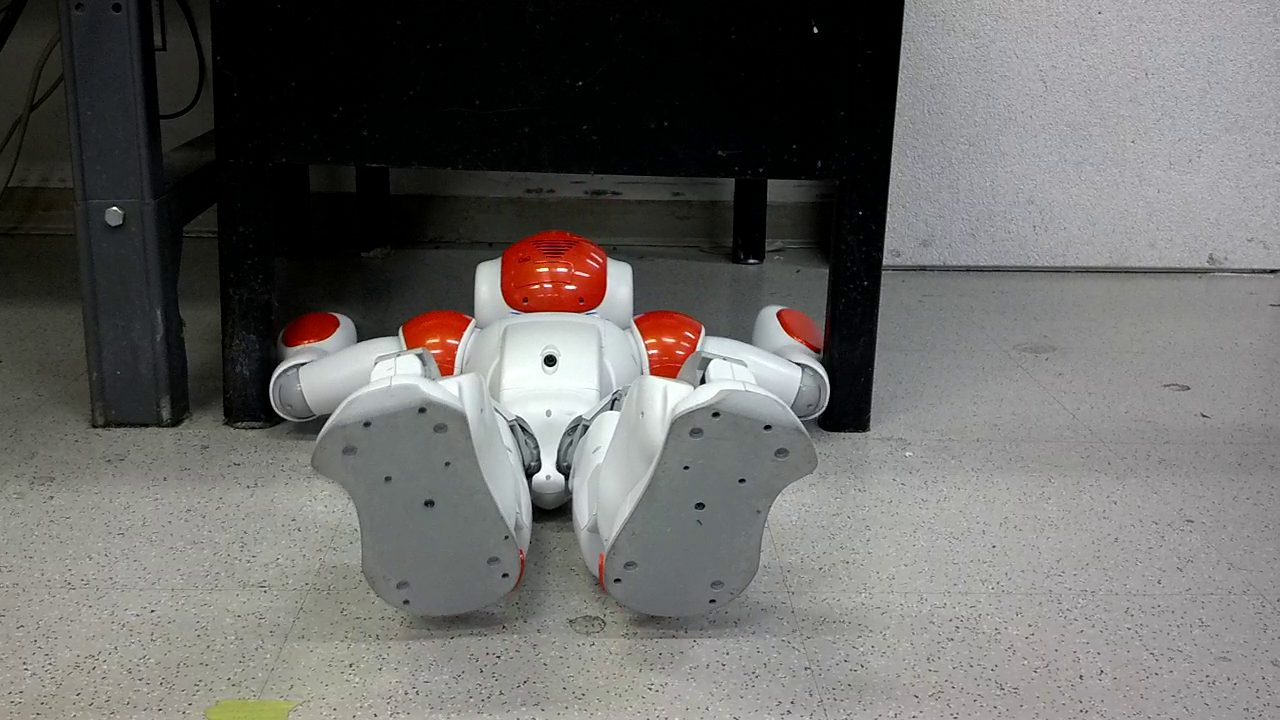
\includegraphics[width=0.25\textwidth]{crawl/under_table/14s.png}
    \includegraphics[width=0.25\textwidth]{crawl/under_table/18s.png}
    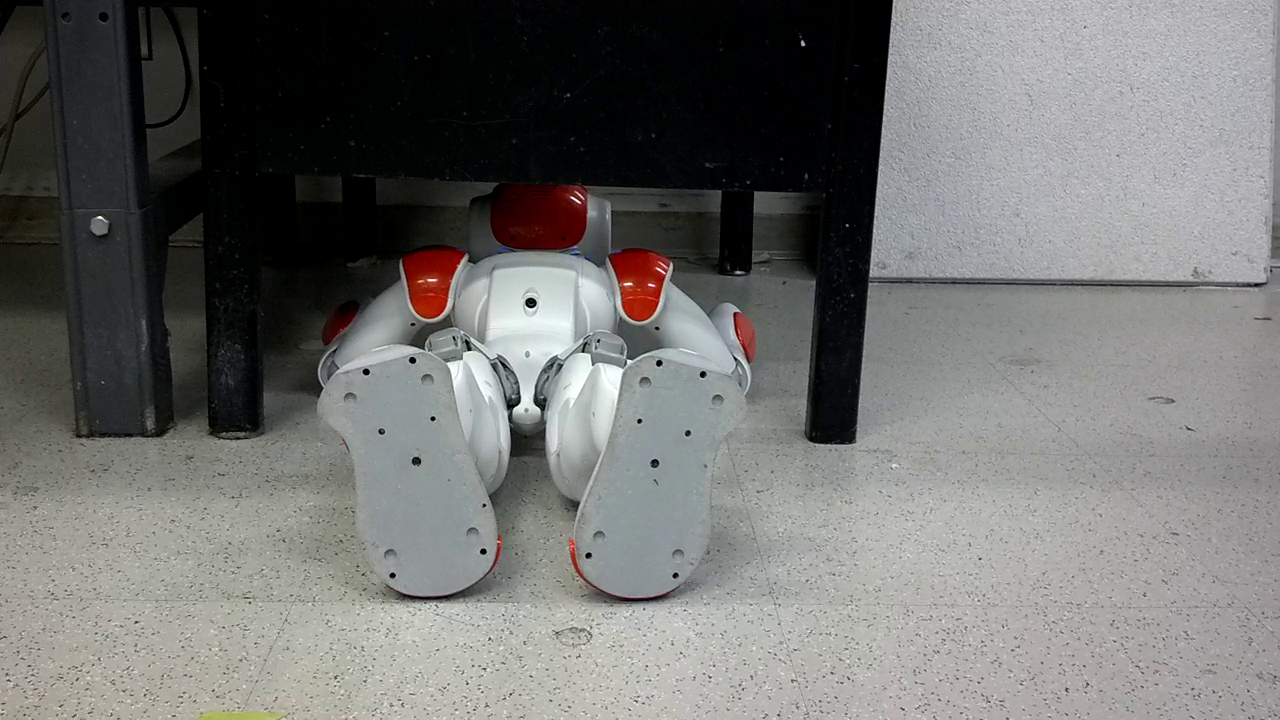
\includegraphics[width=0.25\textwidth]{crawl/under_table/19s.png}
    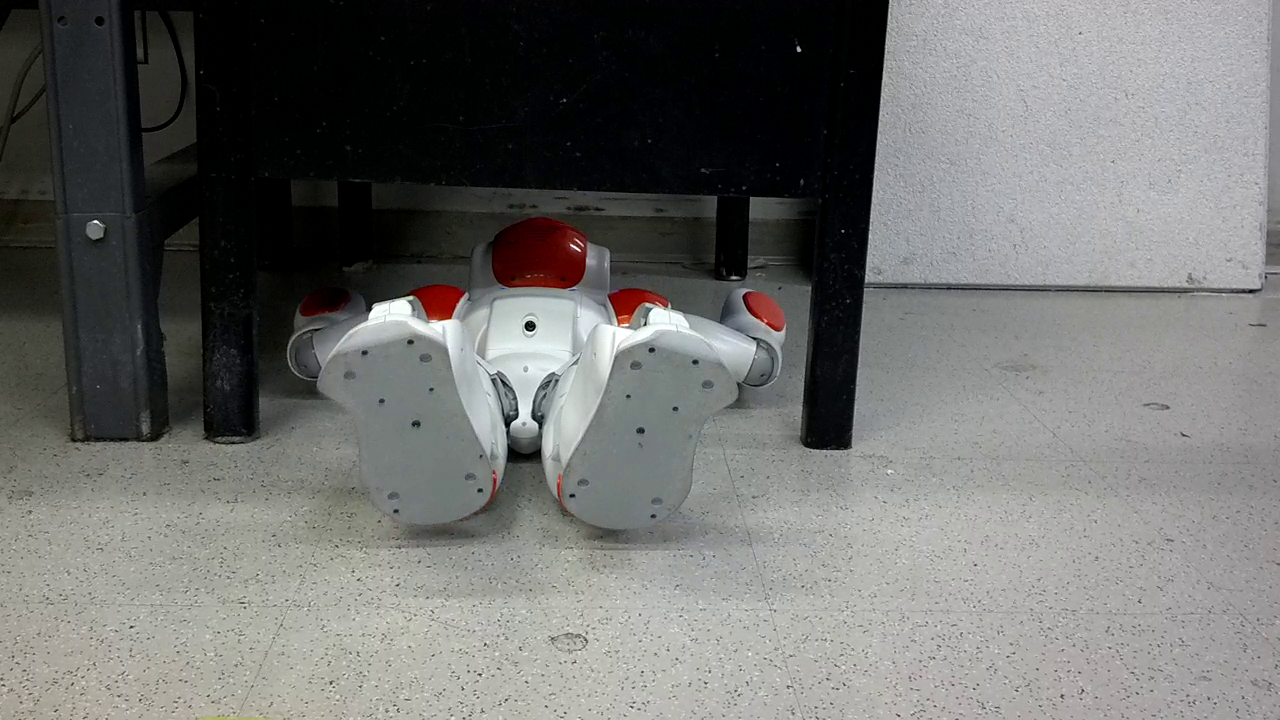
\includegraphics[width=0.25\textwidth]{crawl/under_table/20s.png}
  }
  \caption{Low-profile crawling gait for accessing vertically constrained spaces such as under a table.}
  \label{fig:nao_crawl1}
  \vspace*{-0.07in}
\end{figure}

\begin{figure}
  \centerline{
    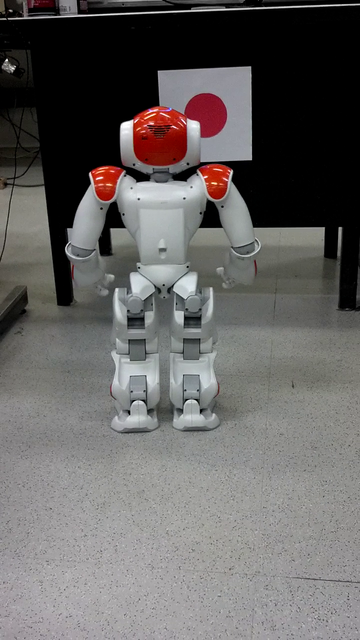
\includegraphics[width=0.2\textwidth]{crawl/walk_to/to/12s.png}
    \includegraphics[width=0.2\textwidth]{crawl/walk_to/to/18s.png}
    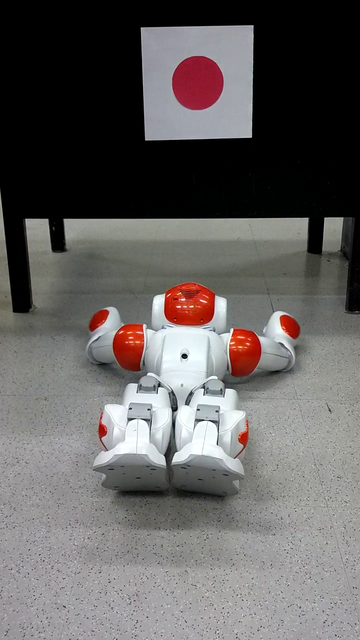
\includegraphics[width=0.2\textwidth]{crawl/walk_to/to/29s.png}
    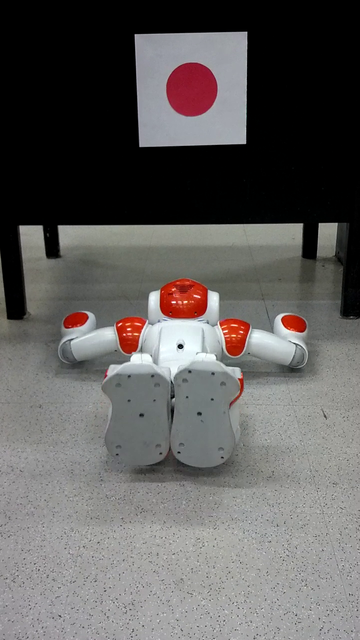
\includegraphics[width=0.2\textwidth]{crawl/walk_to/to/30s_2.png}
    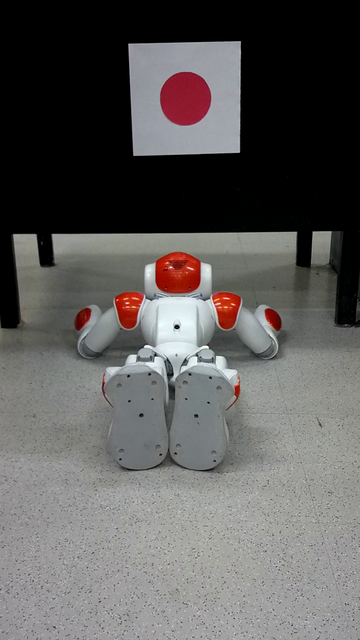
\includegraphics[width=0.2\textwidth]{crawl/walk_to/to/34s.png}
  }
  \vspace*{0.05in}
  \centerline{
    \includegraphics[width=0.2\textwidth]{crawl/walk_to/to/37s.png}
    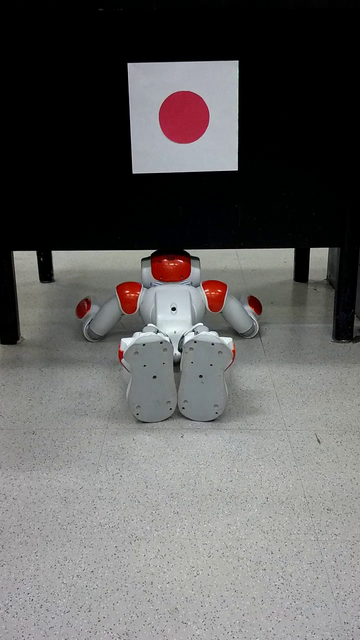
\includegraphics[width=0.2\textwidth]{crawl/walk_to/to/40s.png}
    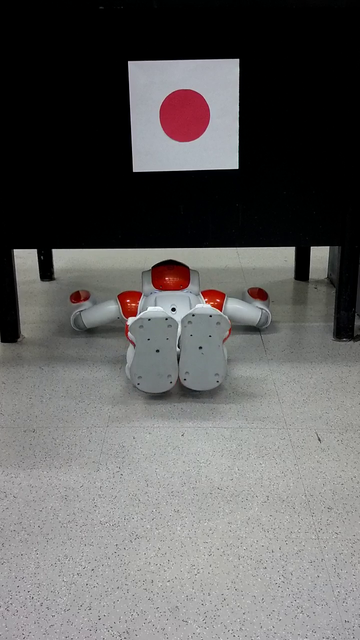
\includegraphics[width=0.2\textwidth]{crawl/walk_to/to/41s.png}
    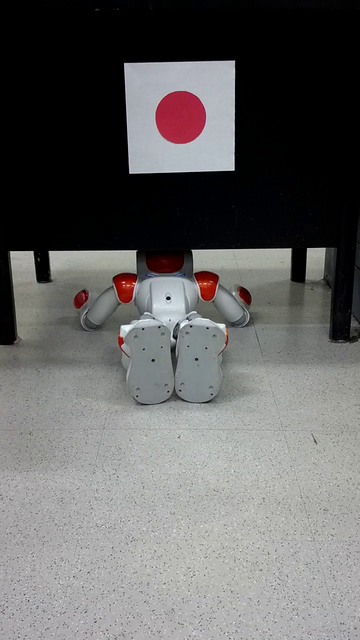
\includegraphics[width=0.2\textwidth]{crawl/walk_to/to/43s.png}
    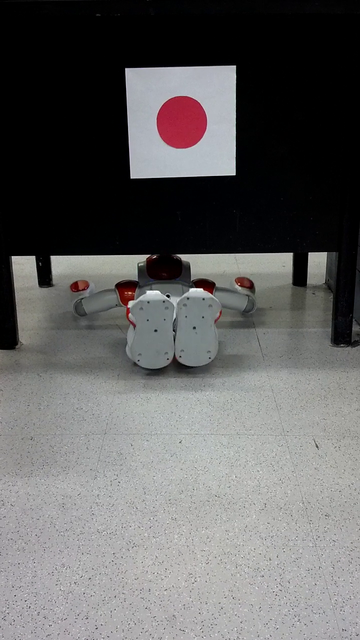
\includegraphics[width=0.2\textwidth]{crawl/walk_to/to/46s.png}
  }
  \vspace*{-0.05in}
  \caption{BLAH BLAH Approaching and crawling under an obstacle.
           A red dot is used as a marker for the direction in which the robot is commanded to move.
           When the robot approaches below a specified distance threshold from the obstacle,
           the crouch-down and crawl gait sequence is initiated.}
  \label{fig:nao_crawl3}
  \vspace*{-0.15in}
\end{figure}

\begin{figure}
  \centerline{
    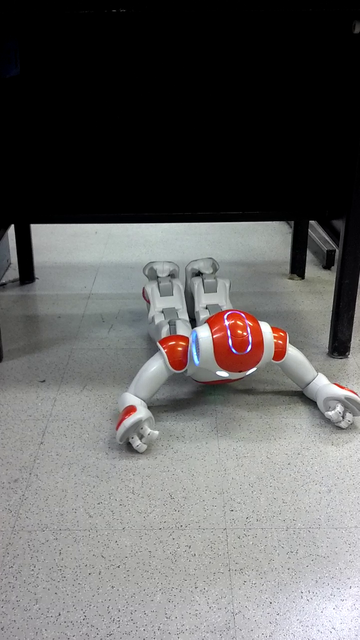
\includegraphics[width=0.2\textwidth]{crawl/walk_to/from/8s.png}
    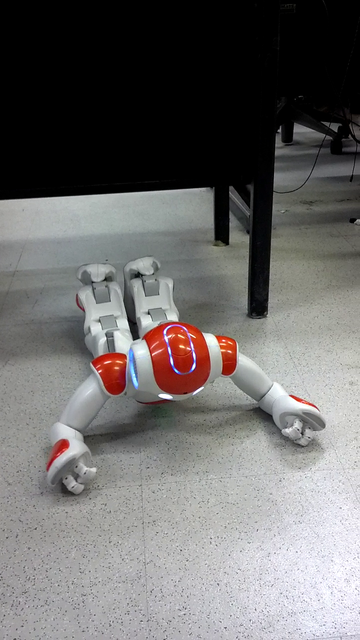
\includegraphics[width=0.2\textwidth]{crawl/walk_to/from/15s.png}
    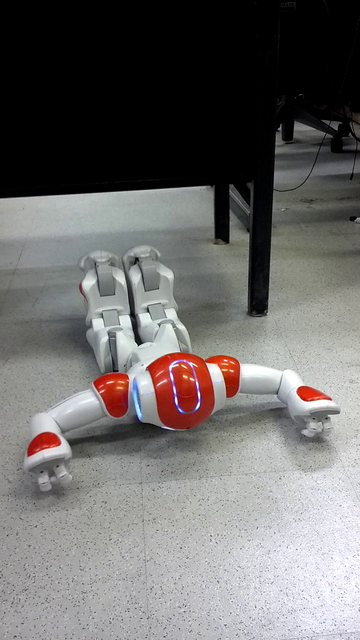
\includegraphics[width=0.2\textwidth]{crawl/walk_to/from/16s.png}
    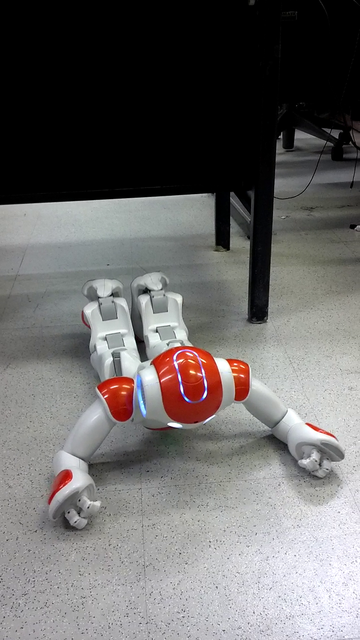
\includegraphics[width=0.2\textwidth]{crawl/walk_to/from/17s.png}
    \includegraphics[width=0.2\textwidth]{crawl/walk_to/from/18s.png}
  }
  \vspace*{0.05in}
  \centerline{
    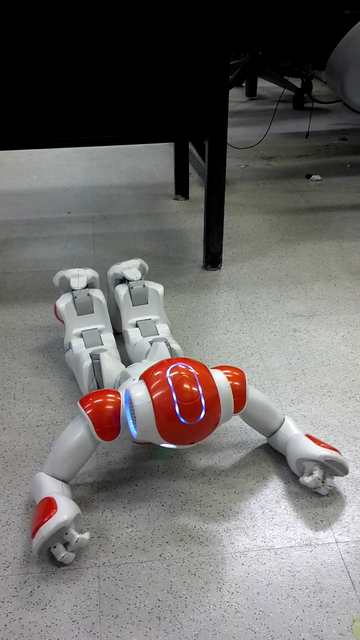
\includegraphics[width=0.2\textwidth]{crawl/walk_to/from/24s.png}
    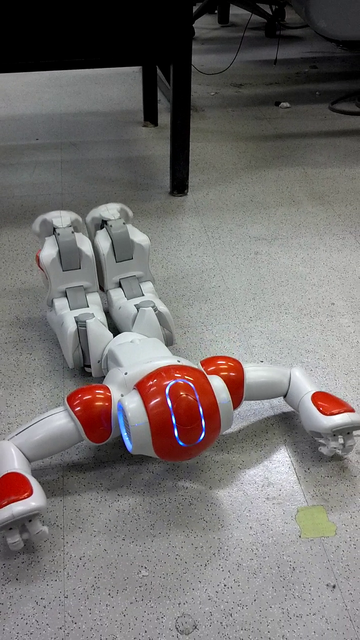
\includegraphics[width=0.2\textwidth]{crawl/walk_to/from/30s.png}
    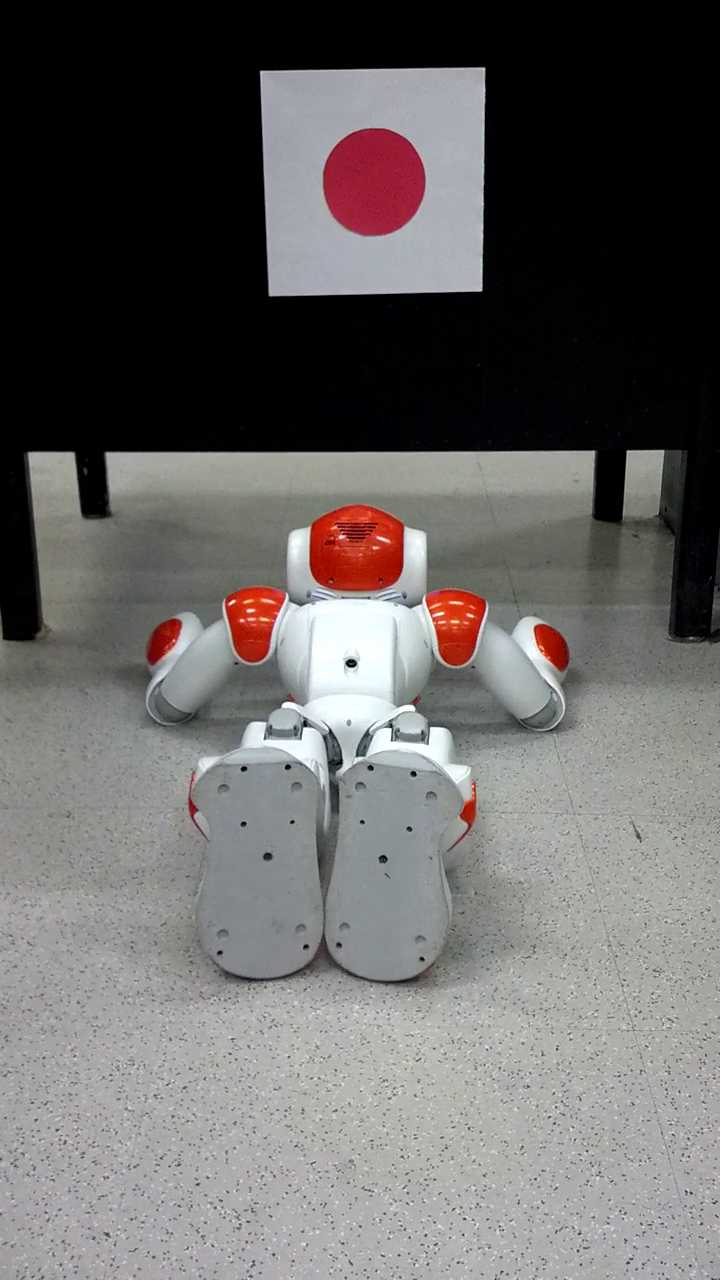
\includegraphics[width=0.2\textwidth]{crawl/walk_to/from/32s.png}
    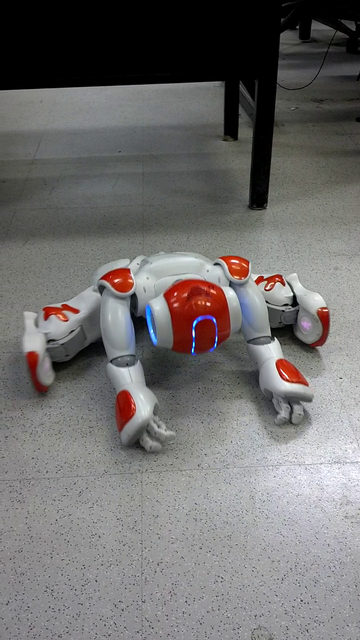
\includegraphics[width=0.2\textwidth]{crawl/walk_to/from/35s.png}
    \includegraphics[width=0.2\textwidth]{crawl/walk_to/from/37s.png}
  }
  \vspace*{-0.05in}
  \caption{BLAH BLAH Crawling under an obstacle and transitioning back to stand posture.}
  \label{fig:nao_crawl4}
  \vspace*{-0.01in}
  \vspace*{-0.05in}
\end{figure}

\begin{figure}
  \centerline{
    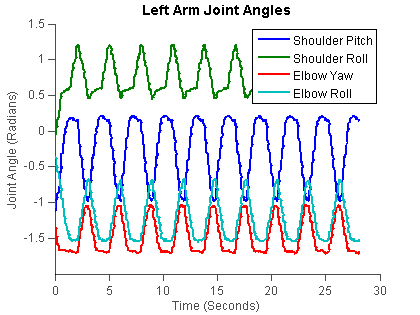
\includegraphics[width=0.5\textwidth]{crawl/joint_angles/LeftArmJointAngles.png}
    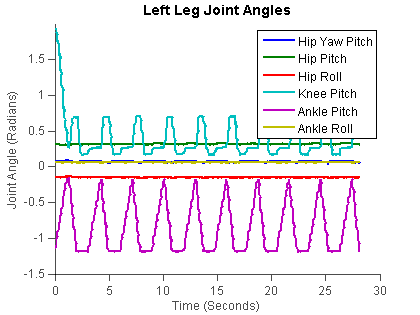
\includegraphics[width=0.5\textwidth]{crawl/joint_angles/LeftLegJointAngles.png}
  }
  \vspace*{-0.05in}
  \caption{Measured motor joint angles during multiple iterations of the periodic crawling gait.
           While the crawling gait is laterally symmetric, the asymmetry in measured angles is due to the
           definitions of the robot frame and joint frame in the NAO API, which essentially forms a mirror
           asymmetry between the left and right joints.}
  \label{fig:nao_joint_angles1}
  \vspace*{-0.1in}
\end{figure}

\begin{figure}
  \centerline{
    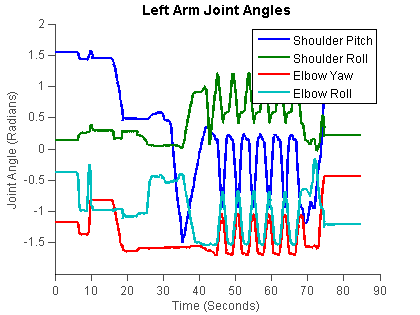
\includegraphics[width=0.5\textwidth]{crawl/joint_angles_long_sequence/LeftArmJointAngles_longSequence.png}
    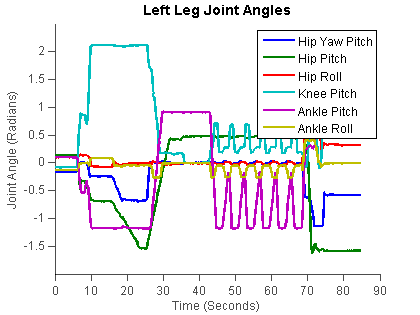
\includegraphics[width=0.5\textwidth]{crawl/joint_angles_long_sequence/LeftLegJointAngles_longSequence.png}
  }
  \vspace*{-0.05in}
  \caption{Measured joint angles for a sequence of transitioning from standing to crouch to crawling,
           crawling under a table, and then returning to crouch.}
  \label{fig:nao_joint_angles_long_seq}
  \vspace*{-0.2in}
\end{figure}

\begin{figure}
  \centerline{
    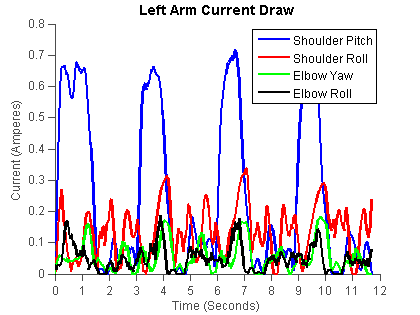
\includegraphics[width=0.5\textwidth]{crawl/current_draws/LeftArmCurrentDraw.png}
    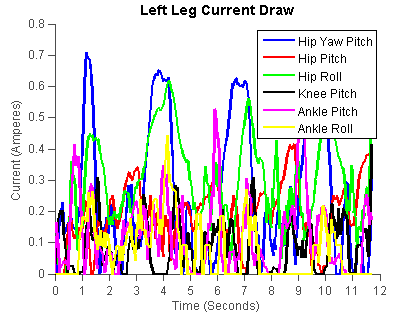
\includegraphics[width=0.5\textwidth]{crawl/current_draws/LeftLegCurrentDraw.png}
  }
  \vspace*{-0.03in}
  \caption{Measured motor current draws during multiple iterations of the periodic crawling gait.}
  \label{fig:nao_currents}
  \vspace*{-0.23in}
\end{figure}


THROW IN A V-REP PICTURE OR 4.


WHAT WERE THE TRIPLET PARAMETERS?

\begin{figure}
  \vspace*{-0.12in}
  \centerline{
    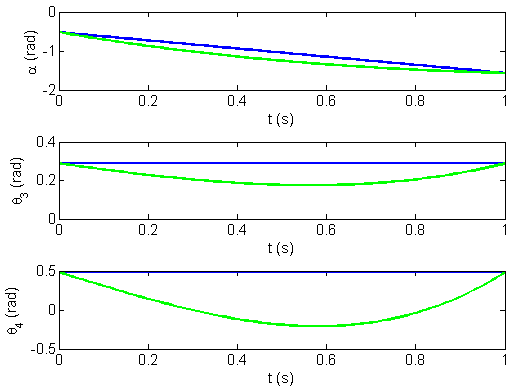
\includegraphics[width=\textwidth]{crawl/cost/ga_cost2_plot1_edit1.png}
  }
  \vspace*{-0.15in}
  \caption{Optimization of crawling motion. Blue lines: nominal time trajectories of the angle triplet 
           $(\alpha,\theta_3,\theta_4)$; Green lines: optimized time trajectories. }
  \vspace*{-0.17in}
  \label{fig:optimal}
\end{figure}
